\documentclass{article}
\usepackage{amsmath}
\usepackage{amssymb}
\usepackage{tikz}
\usetikzlibrary{arrows.meta, positioning}

\begin{document}

\section*{Question 5}

Consider the directed graph $G = (V,E)$ where
\[
V = \{s,a,b,c,d\}
\]
and
\[
E = \{(s,a), (s,b), (a,c), (a,d), (b,c), (b,d)\}.
\]

All edges have equal weight $1$. This graph is shown below.

\begin{center}
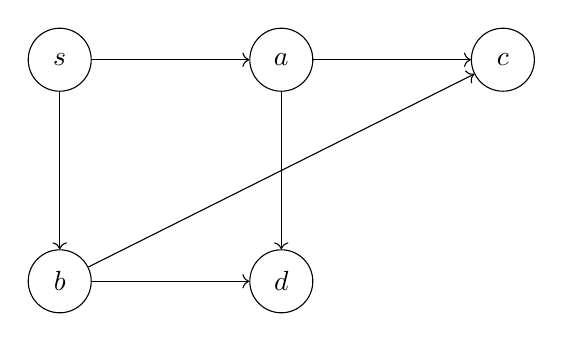
\begin{tikzpicture}[
    node distance=2cm,
    every node/.style={circle, draw, minimum size=8mm},
    every edge/.style={draw, ->}
]

\node (s) {$s$};
\node (a) [right=of s] {$a$};
\node (c) [right=of a] {$c$};

\node (b) [below=of s] {$b$};
\node (d) [right=of b] {$d$};

\draw (s) edge (a);
\draw (s) edge (b);

\draw (a) edge (c);
\draw (a) edge (d);

\draw (b) edge (c);
\draw (b) edge (d);

\end{tikzpicture}
\end{center}

\bigskip

Now define the edge set
\[
E_p = \{(s,a), (s,b), (a,c), (b,d)\}.
\]

This subgraph is shown below.

\begin{center}
\begin{tikzpicture}[
    node distance=2cm,
    every node/.style={circle, draw, minimum size=8mm},
    every edge/.style={draw, ->}
]

\node (s) {$s$};
\node (a) [right=of s] {$a$};
\node (c) [right=of a] {$c$};

\node (b) [below=of s] {$b$};
\node (d) [right=of b] {$d$};

\draw (s) edge (a);
\draw (s) edge (b);

\draw (a) edge (c);
\draw (b) edge (d);

\end{tikzpicture}
\end{center}

\bigskip

\subsection*{Requirement 1}

Each path in $(V,E_p)$ from $s$ to any vertex $v$ is a shortest path in $G$.

\medskip

The shortest path distances in $G$ are:
\begin{align*}
d(s,a) &= 1 \quad \text{via } s \rightarrow a \\
d(s,b) &= 1 \quad \text{via } s \rightarrow b \\
d(s,c) &= 2 \quad \text{via } s \rightarrow a \rightarrow c \text{ or } s \rightarrow b \rightarrow c \\
d(s,d) &= 2 \quad \text{via } s \rightarrow a \rightarrow d \text{ or } s \rightarrow b \rightarrow d
\end{align*}

In $(V,E_p)$, the paths $s \rightarrow a$ and $s \rightarrow b$ have length $1$, while the paths $s \rightarrow a \rightarrow c$ and $s \rightarrow b \rightarrow d$ have length $2$. These path lengths match the shortest path distances in $G$, so Requirement 1 is satisfied.

\bigskip

\subsection*{Requirement 2}

The edge set $E_p$ cannot be produced by a breadth-first search.

Breadth-first search uses a FIFO queue. The execution of this search will be:
\begin{enumerate}
    \item Vertex $s$ is dequeued first, and its neighbors $a$ and $b$ are enqueued.
    \item Next, either $a$ or $b$ is dequeued.
    \begin{itemize}
        \item If $a$ is dequeued first, all of its outgoing edges are discovered, namely to $c$ and $d$. Vertex $a$ becomes the parent of both, resulting in the BFS tree
        \[
        \{(s,a), (s,b), (a,c), (a,d)\}.
        \]
        \item If $b$ is dequeued first, then $b$ becomes the parent of both $c$ and $d$, resulting in the BFS tree
        \[
        \{(s,a), (s,b), (b,c), (b,d)\}.
        \]
    \end{itemize}
\end{enumerate}

In either case, BFS assigns the same parent to both $c$ and $d$. Therefore, it is impossible for $a$ to be the parent of $c$ while $b$ is the parent of $d$, as in $E_p$. Hence, $E_p$ cannot result from a BFS traversal.

\end{document}
